\documentclass[11pt]{article} 
\usepackage{amstex}
\usepackage[dvips]{epsfig}

%included below are the TEX commands
%of Radu Constantinescu, updated 12/20/96

%calligraphic capitals
\newcommand{\iii}{{\mathcal I}}
\newcommand{\jjj}{{\mathcal J}}  
\newcommand{\bbb}{{\mathcal B}}
\newcommand{\lll}{{\mathcal L}}
\newcommand{\ooo}{{\mathcal O}}
\newcommand{\eee}{{\mathcal E}}
\newcommand{\mmm}{{\mathcal M}}
\newcommand{\sss}{{\mathcal S}}
\newcommand{\zzz}{{\mathcal Z}}
\newcommand{\nnn}{{\mathcal N}}
\newcommand{\aaa}{{\mathcal A}}
\newcommand{\ggg}{{\mathcal G}}
\newcommand{\ppp}{{\mathcal P}}
\newcommand{\rrr}{{\mathcal R}}
\newcommand{\uuu}{{\mathcal U}}
\newcommand{\ccc}{{\mathcal C}}
\newcommand{\ddd}{{\mathcal D}}
\newcommand{\fff}{{\mathcal F}}
\newcommand{\kkk}{{\mathcal K}}
\newcommand{\qqq}{{\mathcal Q}}
\newcommand{\ttt}{{\mathcal T}}
\newcommand{\vvv}{{\mathcal V}}
\newcommand{\www}{{\mathcal W}}
\newcommand{\xxx}{{\mathcal X}}
\newcommand{\yyy}{{\mathcal Y}}

%math blackboard letters
\newcommand{\AAA}{{\mathbb A}}
\newcommand{\BBB}{{\mathbb B}}
\newcommand{\CCC}{{\mathbb C}}
\newcommand{\DDD}{{\mathbb D}}
\newcommand{\HHH}{{\mathbb H}}
\newcommand{\KKK}{{\mathbb K}}
\newcommand{\NNN}{{\mathbb N}}
\newcommand{\OOO}{{\mathbb O}}
\newcommand{\PPP}{{\mathbb P}}
\newcommand{\QQQ}{{\mathbb Q}}
\newcommand{\RRR}{{\mathbb R}}
\newcommand{\ZZZ}{{\mathbb Z}}
\newcommand{\SSS}{{\mathbb S}}
\newcommand{\TTT}{{\mathbb T}}

%lowercase Greek letters
\def\a{\alpha}
\def\b{\beta}
\def\g{\gamma}
\def\d{\delta}
\def\e{\epsilon}
\def\vare{\varepsilon}
\def\z{\zeta}
\def\th{\theta}
\def\varth{\vartheta}
\def\i{\iota}
\def\k{\kappa}
\def\l{\lambda}
\def\m{\mu}
\def\n{\nu}
\def\x{\xi}
\def\p{\pi}
\def\varp{\varpi}
\def\r{\rho}
\def\varr{\varrho}
\def\s{\sigma}
\def\vars{\varsigma}
\def\t{\tau}
\def\u{\upsilon}
\def\f{\phi}
\def\varf{\varphi}
\def\h{\chi}
\def\ps{\psi}
\def\o{\omega}

%uppercase Greek letters
\def\G{\Gamma}
\def\D{\Delta}
\def\T{\Theta}
\def\L{\Lambda}
\def\X{\Xi}
\def\P{\Pi}
\def\S{\Sigma}
\def\Ups{\Upsilon}
\def\F{\Phi}
\def\Ps{\Psi}
\def\O{\Omega}

%lowercase fraktur letters
\newcommand{\fa}{{\mathfrak a}}
\newcommand{\fb}{{\mathfrak b}}
\newcommand{\fc}{{\mathfrak c}}
\newcommand{\fd}{{\mathfrak d}}
\newcommand{\fe}{{\mathfrak e}}
\newcommand{\ff}{{\mathfrak f}}
\newcommand{\fg}{{\mathfrak g}}
\newcommand{\fh}{{\mathfrak h}}
\newcommand{\ffi}{{\mathfrak i}}
\newcommand{\fj}{{\mathfrak j}}
\newcommand{\fk}{{\mathfrak k}}
\newcommand{\fl}{{\mathfrakl}}
\newcommand{\fm}{{\mathfrak m}}
\newcommand{\fn}{{\mathfrak n}}
\newcommand{\fo}{{\mathfrak o}}
\newcommand{\fq}{{\mathfrak q}}
\newcommand{\fr}{{\mathfrak r}}
\newcommand{\fs}{{\mathfrak s}}
\newcommand{\ft}{{\mathfrak t}}
\newcommand{\fu}{{\mathfrak u}}
\newcommand{\fv}{{\mathfrak v}}
\newcommand{\fw}{{\mathfrak w}}
\newcommand{\fx}{{\mathfrak x}}
\newcommand{\fy}{{\mathfrak y}}
\newcommand{\fz}{{\mathfrak z}}

%some operatornames
\newcommand{\Spinc}{{\rm Spin}^c}
\newcommand{\Spin}{{\rm Spin}}
\newcommand{\SU}{{\rm SU}\,}
\newcommand{\SO}{{\rm SO}\,}
\newcommand{\U}{{\rm U}\, (1)}
\newcommand{\Endo}{{\rm End}\,}
\newcommand{\cl}{{\rm cl}\,}
\newcommand{\su}{{\rm su}\,}
\newcommand{\Stab}{{\rm Stab}\,}
\newcommand{\Ind}{{\rm Ind}\,}
\newcommand{\Pf}{{\rm Pf}\,}
\newcommand{\Lie}{{\rm Lie}\,}

%shortcuts for some symbols
\newcommand{\doverd}[1]{\frac{d}{d{#1}}}
\newcommand{\partialwrt}[1]{\frac{\partial}{\partial{#1}}}
\newcommand{\half}{\frac{1}{2}}
\newcommand{\vk}{{\vec{k}}}
\newcommand{\vy}{{\vec{y}}}
\newcommand{\vz}{{\vec{z}}}
\newcommand{\vx}{{\vec{x}}}
\newcommand{\vv}{{\vec{v}}}
\newcommand{\vq}{{\vec{q}}}
\newcommand{\rarr}{\rightarrow}
\newcommand{\lrarr}{\longrightarrow}

%shortcuts for TEX commands
\newcommand{\equ}[1]{\begin{equation}{#1}\end{equation}}
\newcommand{\eqs}[1]{\begin{equation*}{#1}\end{equation*}}

%the just-in-case-I-forget part
%1) epsf figures : use xfig, export as eps
%at the top of the latex file say \usepackage[dvips]{epsfig}
%at the insertion point of the figure say
%\begin{center}
%\epsfig{file=filename.eps,width=fraction\linewidth}
%\end{center}
%the fraction is essential since it determines the size
%of the picture (width/total width).






%labels
%sch
%sch0
%eigen
%solsch
%momdis
%inveps
%ls
%intker
%ls2
%ls3
%ampl
 
\begin{document}
  
\begin{center}
{\LARGE\bfseries{Lecture 4: Scattering Theory} }\\
\vskip 1em%
{\Large Edward Witten}\footnote{\tt 
Notes by Radu Constantinescu} 
      \vskip 1.5em%
    {\large December 1996} \\ 
\end{center}


\begin{abstract}
This lecture is an introduction to Scattering Theory
in Quantum Mechanics.
After introducing the asymptotic conditions and explaining their
interpretation in terms of observable quantities, we introduce the 
Lippmann-Schwinger equation and the Born approximation. We then discuss
Feynman diagrams and some differences between
the non-relativistic and relativistic propagation of signals and 
particles.

\end{abstract}

\section{\bf Non-relativistic scattering theory}

\subsection{\bf The asymptotic conditions.}
We start by considering a particle of mass $m$ 
moving in $\RRR^3$ in the time-dependent
potential $V(\vx,t)$ (whose support is not a priori assumed to be localized
in the spatial directions). The evolution of the wave function
$\psi (\vx,t)$ is determined by the time-dependent Schr\"{o}dinger equation
\equ{\label{sch} i\partialwrt{t} \psi (\vx,t) = H\psi (\vx,t),}
where the Hamiltonian is defined by $H=-\frac{1}{2m} \Delta_x + V$. We will
assume for a while that $m=1$.

We want to analyse the solutions of (\ref{sch}) with a certain behaviour
in the far past and the far future. In the far past, we require that
the solutions approach, as $t\rightarrow -\infty$, a solution
of the Schr\"odinger equation corresponding to the {\em free} Hamiltonian
$H_0= -\half \Delta$. Solutions of the free Schr\"odinger equation have the
general form
\equ{ \label{sch0} \psi (\vx,t) = \int \frac{d^3 \vk}{(2\p )^3} f(\vk) 
e^{i (\vk\cdot \vx -\frac{k^2}{2 } t)}, }
where $f(\vk)$ represents the distribution of momenta at time $t=0$.
More specifically, we want to consider those solutions of (\ref{sch0})
corresponding approximately to an incoming particle with velocity $\vv$, which
means that $f(\vk)$ is localized near $\vk_0 = \vv$ (since m=1); a possible
choice for $f$ is 
\equ{\label{momdis} f(\vk )= \exp (-\frac{1}{\a} (k-k_0 )^2 ) }
with small $\a$.
For large $t$, the integral in (\ref{sch0}) is highly oscillatory so the main
contribution comes from stationary phase; varying the exponent with
respect to $k$ gives $\vk = \vx /t$; if $\a$ is small then $\vk$
has to be close to $k_0$, and the condition $\vx=\vk_0 t$ does indeed describe
a free moving particle with velocity $\vk_0$.

In the far future, we can no longer expect the wave function $\psi$ to be 
localised near a definite momentum because of the scattering effect of the
potential, so we will instead look for solutions of (\ref{sch})
which behave asymptotically like a sum of a localised solution of (\ref{sch0})
and an outgoing spherical wave.

In order to find solutions of (\ref{sch}) we will first solve an eigenvalue
problem for the Hamiltonian. 
 We assume that there are no bound states, i.e. that 
$H$ has no discrete spectrum. For each $\vk$ we will search for a solution
${\psi_\vk} (\vx )$ of the equation $H {\psi_\vk} (\vx ) = \frac{k^2}{2}
{\psi_\vk} (\vx )$ with the following asymptotic behaviour at large
distances:

\equ{ \label{eigen} {\psi_\vk} (\vx ) \stackrel{x\rarr\infty}{\lrarr}
e^{i\vk\cdot\vx } +\frac{1}{|x|} e^{i|k|\,|x|} F_\vk (\O ) + 
O \left( \frac{1}{|x|^2}
\right) .
}
The plus sign in the exponent of the second term is important, it will be
needed in the construction of an {\em outgoing} wave solution of (\ref{sch}).
The complex-valued 
function $F_\vk$ is defined on the sphere of radius $1$ and
the notation $\O$ is a shorthand for a vector $\hat{x}$
on the sphere. Alternatively we can regard $F_\vk$ as 
a function $F(\vk^\prime ,\vk )$ defined
for $|\vk^\prime |= |\vk |$.

The functions $\psi_\vk$ can be used to construct exact solutions
of the time-dependent Schr\"odinger equation, namely
\equ{ \label{solsch} 
\psi (\vx, t) = \int \frac{d^3 \vk}{(2\p )^3} f(\vk ) \psi_\vk e^{-i
\frac{k^2}{2} t} .
}
Let us use (\ref{eigen}) and (\ref{solsch}) to see how does $\psi$ look at
infinity if $f$ is assumed to be of the form (\ref{momdis}). For $|t|\rarr\infty$
and $|x|\rarr\infty$ two terms contribute to the stationary phase; one of
them is $\exp i(\vk\cdot\vx - k^2 t/ 2 )$ and has already been analysed--
the stationary phase condition is $\vx = \vk_0 t$. The other one has, for large
$|\vx|$, the phase $|\vk|\cdot |\vx|- k^2 t/2 + \arg F$; varying with respect to $|k|$ we find
 that the stationarity condition is
\equ{  x= kt + \partialwrt{k} \arg F_\vk }

Notice that if we ignored the term involving $F$ we would get $x=kt$, which
cannot be satified for negative $t$-- in agreement with the fact that we only want
to have an {\em outgoing} spherical wave.

The extra term in the right-hand side is a finite time
advance or delay describing the fact that the moment when
the scattered particles arrive at a detector is affected by the 
interaction with the target. The stationarity condition shows that
the advance/delay is the radial derivative of the phase of $F$,
called the {\em phase shift}.

\subsection{\bf Relation with experiments.}
It is now time to relate the above constructions to quantities which are
actually measurable in scattering experiments. The function $F(\O )$ is 
called the {\em scattering amplitude}. The reason for this is that 
the measure $|F(\O )|^2 d^2\O$ on the sphere $S_1=\{ |x|=1 \}$
can be interpreted as the number of scattered particles per unit solid angle
if there is one incident particle per unit area ($d^2 \O $ denotes the
usual measure on the 2-sphere). Notice that only the absolute value of $F$ is
relevant here.
The integral 
\equ{ \s= \int_{S_1} |F(\O )|^2 d^2\O }
is called the {\em total cross-section} and represents the total number
of scattered particles (per unit incoming particle in unit area). As such,
$\s$ can also be viewed as the {\em effective cross-sectional area} of
the target: if the target is thought to remove a fraction of the incoming
particles of momentum $\vk_0$, then $\s$ is the total number of removed
particles if there is one particle per unit area. The relationship
between $\s$ and $F$ is usually written as
\equ{ \frac{d\s}{d\O} = | F( \O )|^2. }


\subsection{\bf The Lippmann-Schwinger equation.}\nopagebreak We have so far
used the eigenfunctions of the Hamiltonian to solve the time-dependent
Schr\"odinger equation. The question now is how to solve the eigenvalue problem
for $H$. One possibility is to start from the free Hamiltonian $H_0= -\half
\D$ whose eigenfunctions are $\exp (i\vk\cdot\vx )$ (corresponding to the
eigenvalues $k^2/2$). We will search for eigenfunctions $\psi_\vk$ of $H$
of the form $\psi_\vk = \exp (i\vk\cdot\vx ) + \a_\vk$. Since $H= H_0 + V$
we have
\equ{ 0=\left( H-\frac{k^2}{2} \right)\psi_\vk = V\psi_\vk +  
\left( H_0 -\frac{k^2}{2} \right) \a_\vk }
which implies
\equ{\label{ls} \a_\vk = -\frac{1}{H_0 -\frac{k^2}{2}} V\psi_\vk , }
where the operator $1/(H_0 - k^2/2 )$ is supposed to be a right-inverse
to $H_0 - k^2/2$.

 Although the operator $H_0 - k^2/2$ is not invertible, we still can 
construct a right-inverse of it
In momentum space, for instance, the operator $H_0 - k^2/2$ is roughly
speaking a multiplication operator
\equ{ \left( H_0 -\frac{k^2}{2} \right) e^{i\vq\cdot\vx} =
\half (q^2 -k^2 )e^{i\vq\cdot\vx} }
so we should have
\equ{ \frac{1}{H_0 -\frac{k^2}{2}}= \frac{1}{\half (q^2 -k^2 )} .}
Because of the pole, there are several ways of making sense of the above;
one possibility, in the usual notation, is:
\equ{\label{inveps}
 \frac{1}{H_0 -\frac{k^2}{2}}= \frac{1}{\half (q^2 -k^2 )-i\e} .}
The conversion to position space is realised through the following

{\bf Exercise.} Show that the integral kernel (in position
space) of the operator defined
 by (\ref{inveps}) is
\equ{\label{intker} G(\vx,\vy) = \frac{1}{2\p} 
\frac{e^{i|k|\cdot|x-y|}}{|x-y|}. }

By using the exercise, (\ref{ls}) leads to the {\em Lippmann-Schwinger equation}
\equ{\label{ls2}\psi_\vk (\vx ) = e^{i\vk\cdot\vx}-\frac{1}{2\p} \int d^3 \vy
\frac{e^{i|k|\cdot|x-y|}}{|x-y|} V(\vy ) \psi_\vk (\vy ). }
If the potential $V$ has compact support then any solution of (\ref{ls2})
has the boundary conditions required by the asymptotic condition built in. This
can be seen by using the fact that for large $|x|$ and $\vy$ in a compact set
we have $|x-y|= |x|- \hat{x}\cdot \vy + O(1/|x| )$, where $\hat{x}= \vx/ |x|$. 
Indeed, if we use this approximation then (\ref{ls2}) becomes
\equ{ \label{ls3}\psi_\vk (\vx ) = e^{i\vk\cdot\vx}-\frac{1}{2\p}
\frac{e^{i|k|\cdot |x|}}{|x|} \int d^3 \vy e^{-i|k|\,\hat{x}\cdot\vy} V(\vy )
\psi_\vk (\vy ) + O\left( \frac{1}{x^2} \right) , }
which shows the existence of a scattered wave of the promised type. 

{\bf Remark.} The procedure used in (\ref{inveps}) for going around the pole
is chosen precisely in order to guarantee the existence of the outgoing
spherical wave.

Notice that (\ref{ls3}) gives an expression for the scattering amplitude: for any
point $\O = \hat{x}$ on the sphere of radius $1$ we have
\equ{\label{ampl}
 F(\O )= -\frac{1}{2\p} \int d^3 \vy e^{-i|k|\,\hat{x}\cdot\vy} V(\vy )
\psi_\vk (\vy ) .}

{\bf Remark.} We can reinterpret the function $F$ as a function of
$k^\prime$ and $k$ such that $|k^\prime | = |k|$, in agreement with the 
idea that after scattering the particle moves in the $\hat{x}$ direction
with the same speed as before.

Although the Lippmann-Schwinger equation cannot be solved exactly, it can be used
to compute $\psi_\vk$ in perturbation theory as an expansion in the powers of
the potential (assumed to be sufficiently weak). This can be done by an iterative
procedure: we first calculate $\psi_\vk$ to order $V$ by using the
free eigenfunction $\exp (i\vk\cdot\vy )$ in the right-hand side of (\ref{ls2})
instead of $\psi_\vk (\vy )$;
once we know $\psi_\vk$ to order $V$ we plug it back into (\ref{ls2})
to get the answer to order $V^2$ and so on.

\subsection{The Born approximation.}
We have seen above an expression of the scattering amplitude in terms of
the eigenfunctions $\psi_\vk$. The {\em first Born approximation} is the 
computation of the scattering amplitude with $\psi_\vk$ replaced in (\ref{ampl}) by
the free plane
wave $\exp (i\vk\cdot\vy )$. We have seen that the scattered wave travels with
the same speed as the incoming one so we can write, for $|\vk^\prime |= |\vk|$,
\equ{ F(\vk^\prime ,\vk ) =
-\frac{1}{2\p} \int d^3 \vy e^{-i \vk^\prime\cdot\vy} V(\vy )
\psi_\vk (\vy ) . }
In the first Born approximation this becomes 
\equ{ F(\vk^\prime ,\vk )_{Born} =
-\frac{1}{2\p} \int d^3 \vy e^{-i (\vk -\vk^\prime )\cdot \vy} V(\vy ) .}
If we introduce the {\em momentum transfer} $\vq = \vk^\prime -\vk $ we see
that $F(\vk^\prime ,\vk )_{Born}$ is the Fourier transform of the potential
in the $\vq$ variable.

{\bf Remark.} This fact is important since it shows that the less smooth
$V$ is, the less rapidly does $F(\vk^\prime ,\vk )$ decay as a function
of $\vk^\prime -\vk $ (for fixed $\vk$). This led Rutherford to postulate
the existence of the atomic nucleus (based on his scattering experiments). 
Later on, when similar experiments were performed with
protons instead of atoms, the same reasoning suggested the composite structure
of the proton (existence of quarks).

 There are also higher Born approximations
for the transition amplitudes: it is enough to use the successive 
approximations to $\psi_\vk$ in the expression (\ref{ampl}) of $F(\vk^\prime ,\vk )$.
It turns out that in general the Born approximations lead to very precise
computations.

{\bf Remark.} Instead of considering a particle incident on a target we can
regard our previous discussion as a description of the interaction
of two particles.
The center of mass decouples and the same results go through for the relative
motion of the particles.

{\bf Remark.} We can also generalize the preceding arguments for the case 
of $n$ interacting particles. Let us note that this time we won't be able to
simultaneously normalize the masses to $1$ and that we need one spherical
wave centered at each interaction point. The exact solutions of the
Schr\"odinger equation $\psi_{\vk_1 ,\ldots, \vk_n }$
will be sums of free and spherical waves away from the diagonals (i.e.
whenever $\vk_i \neq \vk_j$ for $i\neq j$).

\subsection{Feynman diagrams.}
Starting from (\ref{ampl}) and the Lippmann-Schwinger equation we can compute
the transition amplitude as an infinite sum
\begin{eqnarray*}
F(\vk^\prime ,\vk ) & = & -\frac{1}{2\p }\int d^3 \vx e^{-i (\vk^\prime -\vk )
			 \cdot\vx} V(\vx ) \\
		   &   & +\frac{1}{4\p^2} \int d^3 \vx d^3 \vy e^{-i\vk^\prime\cdot
			 \vx} V(\vx) G(\vx, \vy )V(\vy) e^{i\vk\cdot\vy} \\
		   &   & -\frac{1}{8\p^3} \int d^3 \vx d^3 \vy d^3 \vz
			 e^{-i\vk^\prime\cdot\vx} V(\vx) G(\vx, \vy )V(\vy)
			 G(\vy, \vz )V(\vz) e^{i\vk\cdot\vz} \\
		   &   & +\cdots
\end{eqnarray*}

Given our experience with Feynman diagrams, it is easy to see that the terms of the sum
can be represented graphically (for instance, the graphs corresponding to the
first three terms in the sum are shown below).

\begin{center}

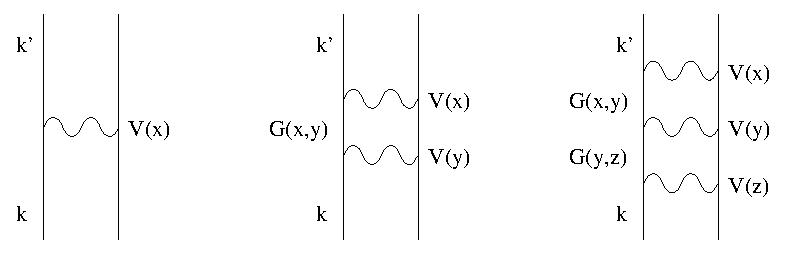
\epsfig{file=witt4fig1.eps,width=.8\linewidth}

\end{center}

Each curly line represents an interaction due to the potential $V$. In-between
interactions, the particles move freely (hence the free propagator
$G(x,y)$). The incoming and outgoing particles have definite momentum
($\vk, \vk^\prime $, respectively). The diagrams can be thought to encode
either the relative motion of two particles or the evolution of one
particle scattered by a fixed target. Notice that only very simple
(ladder) diagrams appear, corresponding to that fact that there
are no creation/annihilation phenomena in this non-relativistic
description.

\section{Relativistic versus non-relativistic scattering theory}

We will now analyse some differences between the non-relativistic
picture we have been considering so far and the 
relativistic treatment of scattering theory. 
\subsection{Propagation of particles}
Going back to the time-dependent Schr\"odinger equation (\ref{sch}), we can try 
to solve it directly by imitating the method used in 1.3
to derive the Lippmann-Schwinger
equation. We can use the plane
wave solutions $\exp i(\vk\cdot\vx -\frac{k^2}{2} t)$ of the {\em free}
Schr\"odinger equation to transform the Schr\"odinger equation for $H$
into an integral equation: any solution of the perturbed Schr\"odinger equation
satisfies the following analogue of Lippmann-Schwinger:
\equ{ \label{solsch2} \psi = e^{ i(\vk\cdot\vx -\frac{k^2}{2} t)}
-\frac{1}{i\partialwrt{t} -\half \D} V\psi .}
As in Subsection 1.3., the easiest way of making sense of the inverse
of $i\partialwrt{t} -\half \D$ is in momentum space. Since
\equ{ \left(    i\partialwrt{t} -\half \D   \right)
 e^{i(\vq\cdot\vx -E t)} =\left( E-\frac{q^2}{2} \right) 
e^{i(\vq\cdot\vx -Et)},   }
an inverse (in momentum space) can be found by prescribing the way to go around
the pole $E=q^2 /2$. For instance, we could use
\equ{\frac{1}{i\partialwrt{t} -\half \D} e^{i(\vq\cdot\vx -E t)}=
\frac{1}{E-\frac{q^2}{2} +i\e} e^{i(\vq\cdot\vx -E t)} .}
The integral kernel of the chosen inverse, in position space, is given by
the inverse Fourier transform
\equ{ G(\vx,t;\vx^\prime, t^\prime )=\int \frac{d^3\vq}{(2\p )^4} 
e^{i\vq\cdot\vx}
\int_{-\infty}^{\infty} dE \frac{e^{-iE (t-t^\prime )}}{E-\frac{q^2}{2} +i\e} .}

The only pole of the $E$ integral is at $E=\frac{q^2}{2} - i\e$ and so,
{\em if} $t-t^\prime < 0$ we get $G=0$(because we can then avoid
the pole by closing the integration
contour in the upper half-plane). This result has an important
implication:
{\em particles can only travel forward in time}.

This is no longer true in a relativistic context: we have seen that
the typical propagator of a particle of a mass $m$ is
$$\frac{1}{q_0^2 -\vq^{\, 2} + m^2 +i\e} $$
in momentum space; in position space, the inverse Fourier transform gives
(for $x= (\vx, t))$
\equ{ G(x, x^\prime)=\int \frac{d^3\vq}{(2\p )^4} 
e^{i\vq\cdot\vx}
\int_{-\infty}^{\infty} dE \frac{e^{-iE (t-t^\prime )}}{q_0^2-\vq^{\, 2} +m^2 +i\e} .}
No matter whether we close the integration contour in the upper or lower
half-plane, we cannot avoid both poles, therefore
it is no longer true that $G$ vanishes if the time coordinates of the
points $x$ and $x^\prime$ satisfy $t<t^\prime$. As a consequence,
particles can make zig-zags in time, a phenomenon which is
interpreted as the creation or annihilation
of particle/antiparticle pairs (the particles traveling forward in time
and the antiparticles backwards).

\subsection{Propagation of signals}

Non-relativistically, interactions are instantaneous. However, this is no
longer true in the relativistic case.

 Let us consider the example of the electromagnetic field; the 
interaction is transmitted by photons traveling at the speed of light
(since the interaction is not instantaneous,
we model it by some particles
moving at finite speed).

The photon propagator in momentum space equals $1/ (q_0^2 - \vq^{\, 2} +i\e )$, 
an expression whose
non-relativistic limit (given by $q_0\rarr 0$)
 is formally $-1/\vq^{\, 2}$. This has to be reinterpreted since
non-relativistically there is no creation and annihilation of particles
(so the only way we can think about the photon non-relativistically
is to consider that it only exists at the time $t_0$ when the interaction
occurs).

Notice that the (four-dimensional) inverse Fourier transform of $-1/\vq^{\, 2}$ equals
\equ{  -\int \frac{d^4 q}{(2\p )^4} \frac{e^{iq\cdot y}}{\vq^{\,2}} =-\d (t)\frac{1}{|\vy |}, }
which is precisely a delta-function in time multiplied by the Coulomb potential.
Therefore the non-relativistic limit corresponds to an {\em instantaneous} interaction
(i.e. scattering in the Coulomb potential). Relativistically, 
\equ{  -\int \frac{d^4 q}{(2\p )^4} \frac{e^{iq\cdot y}}{q_0^2 -\vq^{\, 2} +i\e} }
is no longer supported at a fixed point in time, so the interaction
is not instantaneous.

We can also illustrate the results on the propagation of particles
and interactions in perturbation theory. It was shown that non-relativistically
only ladder diagrams are encountered; intuitively, if time flows in the
vertical direction, these diagrams represent particles moving forward
with the horizontal curly lines being instantaneous interactions.

\begin{center}

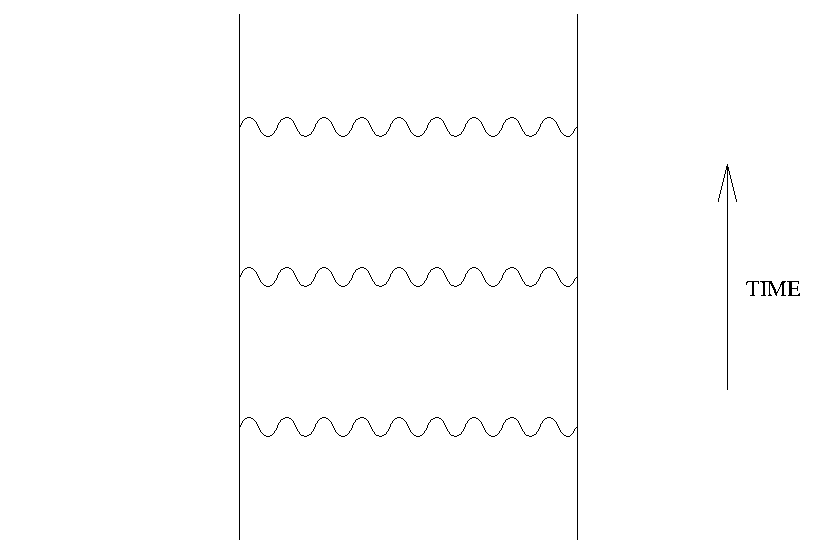
\epsfig{file=witt4fig3.eps,width=.3\linewidth}

\end{center}

By contrast, in the relativistic case interactions travel at the speed of light
and particle/antiparticle pairs can appear, so more complicated Feynman
diagrams such as the ones below have to be considered.


\begin{center}

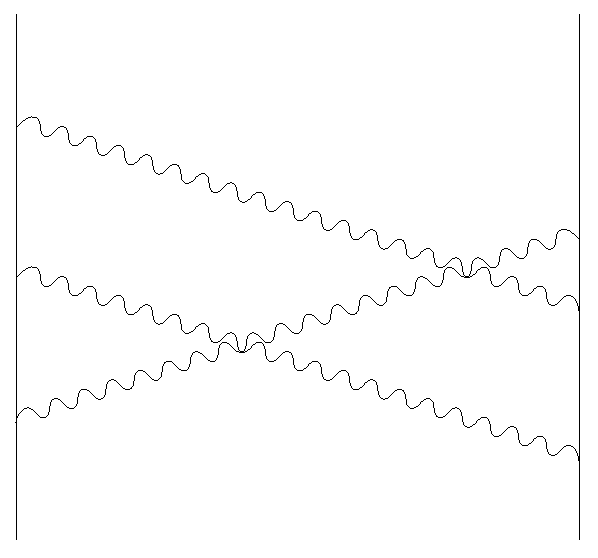
\epsfig{file=witt4fig2.eps,width=.3\linewidth}

\end{center}

This diagram illustrates the fact that photons traveling at the speed of light
replace the non-relativistic instantaneous interaction. The curly line
which represents the interaction in the non-relativistic case is relativistically
a photon.
In the second diagram
we show the creation and annihilation of particle pairs. (Of course there
are also diagrams in which both effects are present.) The diagram also illustrates
another important fact:
in a local theory,
the presence of electron/positron pairs makes it impossible
to count `the total number of particles in the universe'. The totality of
electrons can be accounted for by a single electron zig-zagging in time or even
a sigle closed loop.



\begin{center}

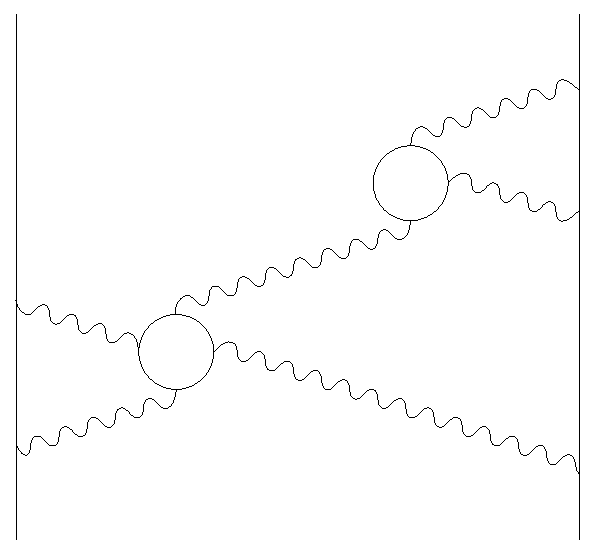
\epsfig{file=witt4fig4.eps,width=.3\linewidth}

\end{center}

 The diagram also illustrates
another important fact:
in a local theory,
the presence of electron/positron pairs makes it impossible
to count `the total number of particles in the universe'. The totality of
electrons can be accounted for by a single electron zig-zagging in time or even
a single closed loop.

\begin{center}

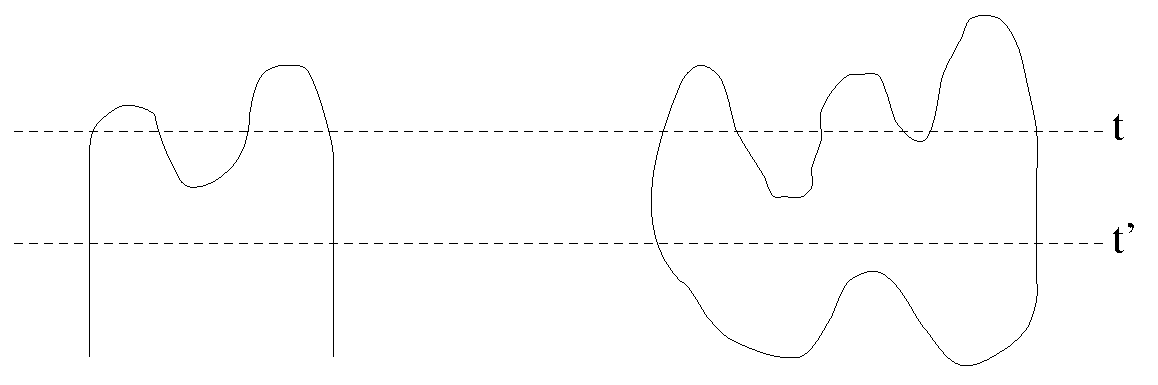
\epsfig{file=witt4fig5.eps,width=.7\linewidth}

\end{center}

\end{document}